\documentclass[a4paper, 11pt]{article}
\usepackage[utf8]{inputenc}
\usepackage{graphicx}
\usepackage{url}
\usepackage{hyperref}
\usepackage{color}
\usepackage{enumitem}

\title{LabSpace: A Collaborative Space where Knowledge and Experience is Shared}
\author{George E. Kallergis\\geokal@kth.se}
\date{\today{}}

\begin{document}

\maketitle

\begin{figure}[h!]
  \begin{center}
    
\includegraphics[width=\textwidth,height=\textheight,keepaspectratio]{imagery/logo.png}
    \label{fig:dneaf}
  \end{center}
\end{figure}

\textit{This document describes the benefits and operational model of LabSpace; a collaborative space where students, professors, professionals and enthusiasts can exchange knowledge and experiences on a wide variety of areas including, but not limited to engineering, business, economics and art.}

\newpage

%========%
% Introduction %
%========%
% The introduction gives an overview of the vision and goals of LabSpace as well as its operating environment.
\section*{Introduction}
LabSpace is a specially engineered maker-space \cite{whatsamakerspace} targeting the academic environment where students, professors, professionals and other enthusiasts can meet and exchange theoretical and practical knowledge around a multitude of areas of interest (engineering, business, economics, art etc.). The main vision of LabSpace is to promote the exchange of knowledge and ideas between interdisciplinary teams, sparking innovation and allowing people to make an impact through their abilities. Mentoring, coaching as well as teaching relationships are also encouraged among LabSpace's members.

Figure \ref{fig:ls_env} shows LabSpace inside its preferred context. Preferred context is defined as the ideal environment into which LabSpace is expected to acomplish it's goals in an efficient and sustainable manner. It is beneficial here to explain each of the components in more detail. The \textit{implementing academic organization} is the academic organization (i.e. the university or school) that hosts LabSpace into its premises. The \textit{socioeconomic environment} is the society and the economy into which the \textit{implementing academic organization} operates in. In other words, this block models the country the \textit{implementing academic organization} is in, along with all of its social and financial forces that affect the operation of the later. The \textit{corporations} denote the commercial organizations that are active in that particular \textit{socioeconomic environment}. Finally, the \textit{other academic organizations} block defines other universities or schools that although they are not implementing LabSpace, they contribute to an already existing implementation sharing people and other resources. The actors in Figure \ref{fig:ls_env} define the roles different people play in the different environments inside and outside of LabSpace. 
The different roles outside of LabSpace are explained below:

\begin{itemize}[noitemsep]
    \item \textit{Professor}. The person that is employed as a professor in either the \textit{implementing academic organization} or any \textit{other academic organization}.
    \item \textit{Researcher}. The person that is employed as a researcher in either the \textit{implementing academic organization} or any \textit{other academic organization}.
    \item \textit{Student}. The person that is studying at either the \textit{implementing academic organization} or any \textit{other academic organization}.
    \item \textit{Professional}. The person that is employed by one or more \textit{corporations} (see definition above) and is either representing his/her organization or is contributing to LabSpace as an individual.
    \item \textit{Enthusiast}. The person that belongs to none of the above categories, but still contributes to LabSpace.
\end{itemize}

All of the above roles when active inside of LabSpace, turn into one (or multiple) of the following:

\begin{itemize}[noitemsep]
    \item \textit{Spacer}. The person that is learning and enhancing his/her skills inside LabSpace by participating to projects or being mentored, coached or teached by others.
    \item \textit{Mentor}. The person that is mentoring one or more spacers inside of LabSpace.
    \item \textit{Coach}. The person that is coaching one or more spacers inside of LabSpace.
    \item \textit{Teacher}. The person that is teaching one or more spacers inside of LabSpace.
\end{itemize}

Observing LabSpace from a different perspective, we could see it as a transformation of roles. Inside of LabSpace it doesn't matter if you are a professor or a student, both can teach and both should be open to learning from anybody regardless of the roles they posses outside of LabSpace. It is a neutral zone from the knowledge perspective.

\begin{figure}[h!]
  \begin{center}
    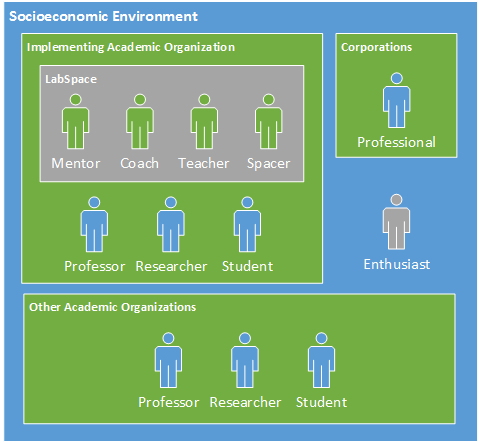
\includegraphics[width=\textwidth,height=\textheight,keepaspectratio]{imagery/ls_context.png}
    \caption{LabSpace into the Preferred Context.}
    \label{fig:ls_env}
  \end{center}
\end{figure}

From the discussion above, we can easily identify the different stakeholders in LabSpace's environment. These are the \textit{implementing academic organization}, the \textit{corporations}, the \textit{other academic organizations} and the individual \textit{professionals} and \textit{enthusiasts} that are active in a LabSpace.

%\begin{quote}
%    \textit{""}
%\end{quote}
%======%
%  Benefits %
%======%
% The benefits section discusses the benefits LabSpace brings to the different stakeholders.
\section{Benefits}
The following sections discuss in more detail how the implementation of a LabSpace can benefit the different entities involved in its operation. In other words the proposed value of a LabSpace is shown and analyzed from the perspective of different stakeholders.

\subsection{Implementing Academic Organization}
\textit{Why is it a good idea for a university to have a LabSpace? How will it benefit from it? What will the university have to do in order to implement a LabSpace? Sponsors? Innovation? Benefits for the international image of the university? Cross university cooperations (i.e. Konstfack)?}

\subsection{Other Academic Organizations}

\subsection{Corporations}

\subsection{Individual Enthusiasts}

\subsection{LabSpace Members}
\textit{How can students benefit from LabSpace? Learning from others that already have the experience? How can that ease their learning curve? Socialize? Network? Share resources and get access to things they couldn't otherwise have access to? Opportunity for startups? Opportunity to teach others? Focus on industry important matters? Benefits on future employment possibilities? Enrich their CV with cool projects?}

%=======%
% Operation %
%=======%
% The operation section discusses the operational model of LabSpace and how an interested academic organization can go about implementing it.
\section{Operation}

\subsection{LabSpace Business Model}
\textit{How will LabSpace be self sustainable? Which are going to be it's partners and the key activities that need to be undertaken in order for it to operate properly? What are the costs (if any) and how are they going to be covered (the less the financial impact on the university the better)?}

\subsection{Space Layout}
\textit{This is specific to the Electrum lab. It consists of a top view of the lab where the placement of available resources (i.e. teables, PCs, other equipment) is shown. The goal is  to allow for  easy concurrent access for the maximum number of students.}

\subsection{Equipment}
\textit{The minimum required equipment for operation will be discussed here and a list specifically for Electrum can be created.}

\subsection{Space Management}
\textit{The "fair use" policy will be defined here to ensure that the space can be used by anyone, but also specific resources can be bound for future use (e.g. breadboards and components to avoid assembly and disassembly of the circuit on every visit). Access to the building will be discussed here.}\cite{mobilehealth}

\newpage

\begin{thebibliography}{9}
    \bibitem{whatsamakerspace} \emph{What’s a Makerspace?} (n.d.) [Online]. Available: \\ \href{http://makerspace.com/home-page}{http://makerspace.com/home-page} (Accessed: February 3\textsuperscript{rd}, 2014).
    
    \bibitem{homeappliances} Mardiana, B. et al., 2009. \emph{"Homes Appliances Controlled Using Speech Recognition in Wireless Network Environment"}, Computer Technology and Development, 2009. ICCTD’09. International Conference on. IEEE, pp.                        
285–288.
    \bibitem{semanticweb} Pathak, J. et al. \emph{"A Framework for Semantic Web Services Discovery."} Artificial Intelligence Research Laboratory, Department of Computer Science, Iowa State University, USA.
    \bibitem{crossreality} Lifton, J. et al. \emph{"Metaphor and Manifestation-Cross-Reality with Ubiquitous Sensor/Actuator Networks."} Pervasive Computing, IEEE 8.3 (2009): 24-33. \copyright 2009 Institute of Electrical and Electronic Engineers.
    \bibitem{mobile} Fling, B. 2009. \emph{"Mobile Design and Development"}, O'Reily, USA, Chapter 4.
    \bibitem{smarthome} Alam, M.R., Reaz, M.B.I. \& Ali, M.A.M., 2012. \emph{"A Review of Smart Homes—Past, Present, and Future"}, Systems, Man, and Cybernetics, Part C: Applications and Reviews, IEEE Transactions on, 2012. IEEE, pp.11905–1203.
    \bibitem{sensornet} Liang, L., 2008. \emph{"Design and implementation of wireless Smart-home sensor network based on ZigBee protocol "}, International Conference on Communications, Circuits and Systems, 2008, ICCCAS 2008. pp. 434–438
    \bibitem{emotionface} Metallinou, A. et al. \emph{"Visual Emotion Recognition Using Compact Facial Representations and Viseme Information"} Department of Electrical Engineering, University of Southern California, Los Angeles, USA.
    \bibitem{solardisposal} Karen, B., Chhaya, G., Shelton, H., Mahshad, Z., 2011. \emph{"Methods and Concerns for Disposal of Photovoltaic Solar Panels"}  Department of General Engineering, San Jose State University, USA.
    \bibitem{mobilehealth} Kevin O’Neill, 2011. \emph{"Mobile phone health risks:
the case for action to protect children"} MobileWise Charity, UK.
    \bibitem{wifi} Kiera Chion, 2011. \emph{"Wi-Fi Health Effects: A 'Full Spectrum' Controversy"}
    \bibitem{pervasivecomp} Satyanarayanan, M. 2001. \emph{"Pervasive Computing: Vision and Challenges"}, IEEE Personal Communications.
\end{thebibliography}

\end{document}
